\documentclass[aspectratio=169,10pt]{beamer}
\usetheme[numbering=fraction,progressbar=none,sectionpage=none,block=fill]{metropolis}
\usepackage[T1]{fontenc}
\usepackage{lmodern}
\usepackage{textcomp}
\usepackage{booktabs,colortbl,tabularx,array}
\usepackage{tikz}
\definecolor{navy}{HTML}{1B2A4A}
\definecolor{muted}{HTML}{5B6577}
\definecolor{good}{HTML}{1E7A60}
\definecolor{bad}{HTML}{B03A2E}
\definecolor{hl}{HTML}{DDEFE8}
\definecolor{routeA}{HTML}{C9731F}
\definecolor{routeB}{HTML}{2F7FC1}
\definecolor{routeC}{HTML}{3E8E57}
\definecolor{routeD}{HTML}{7D5BA6}
\setbeamercolor{frametitle}{bg=navy,fg=white}
\setbeamercolor{title separator}{fg=navy}
\setbeamercolor{normal text}{fg=black!88,bg=white}
\setbeamercolor{alerted text}{fg=good}
\setbeamercolor{block title}{bg=navy!10,fg=navy}
\setbeamercolor{block body}{bg=navy!4}
\setbeamerfont{frametitle}{size=\large,series=\bfseries}
\setbeamertemplate{frame footer}{DocQuorum: agentic document extraction with open models}
\newcolumntype{Y}{>{\raggedright\arraybackslash}X}
\newcommand{\src}[1]{\par\vfill{\tiny\color{muted}#1\par}}
\newcommand{\route}[1]{\tikz[baseline=-0.65ex]\node[circle,fill=route#1,text=white,inner sep=1.3pt,font=\scriptsize\bfseries]{#1};}
\newcommand{\cand}[2]{\tikz[baseline=-0.65ex]\node[circle,fill=#2,text=white,inner sep=1.3pt,font=\scriptsize\bfseries]{#1};}
\newcommand{\nul}{\textcolor{bad}{\texttt{null}}}
\title{DocQuorum}
\subtitle{Agentic document extraction with open models:\\the pipeline on real benchmark documents}
\date{October 2026}
\author{}
\institute{Every example is a real benchmark document and a stored pipeline output; no model was called to make these slides.}
\begin{document}
\maketitle
\section{Task and pipeline}
\begin{frame}{Outline}
\begin{columns}[T]
\column{0.48\textwidth}
\begin{enumerate}
\item Task and pipeline
\item Walkthrough on real documents\\
  {\footnotesize inputs, routing, parsing, readers, deterministic checks, selection by quorum, output}
\item Results on six benchmarks; zoom re-reading
\item Summary
\end{enumerate}
\column{0.48\textwidth}
\begin{block}{Setting}
\small
Open-weight models only: Qwen3.8-27B (FP8) for reading and MinerU2.5 for parsing scans, served on a single GPU.
Each benchmark is scored with its own official scorer.
\end{block}
\end{columns}
\end{frame}
\begin{frame}{Problem statement}
\begin{columns}[T]
\column{0.40\textwidth}
\begin{block}{Task}
\small
\textbf{Input:} a document $D$ (PDF or image), a JSON Schema $S$ or a JSON template, and optionally a task description $T$.\\[0.4em]
\textbf{Output:} one JSON object $Y$ that conforms to $S$, every value supported by $D$, absent values \texttt{null}.
\end{block}
\vspace{0.3em}
{\footnotesize\textbf{Optional task} (real example, receipt schema):\\
\itshape ``A single point-of-sale purchase RECEIPT (retail or restaurant). DOC-TYPE / SCOPE RULE: if one file bundles MULTIPLE \ldots''\par}
\column{0.25\textwidth}
\centering
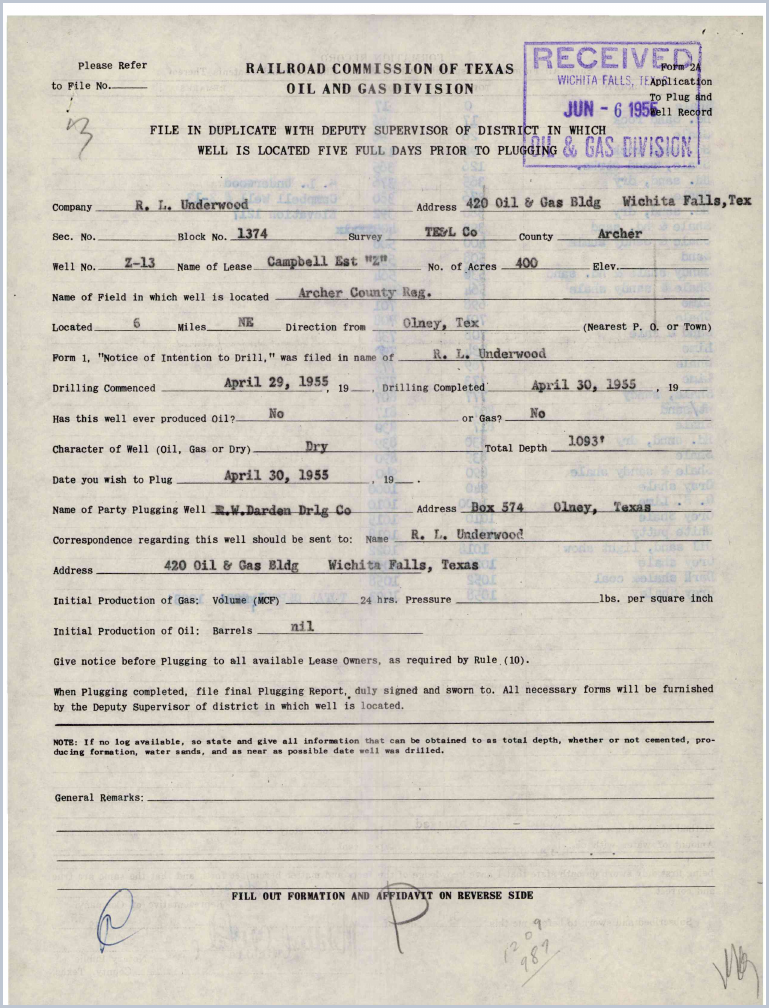
\includegraphics[height=4.2cm]{assets/input_form_p1.png}\\[0.3em]
{\tiny Scanned 1955 well-plugging application (Railroad Commission of Texas), 2 pages, no text layer.\par}
\column{0.33\textwidth}
\textbf{\small JSON Schema (77 fields), excerpt}\\[0.3em]
\begin{beamercolorbox}[wd=\linewidth,sep=0.5em]{block body}
{\tiny\ttfamily\raggedright \textquotedbl{}p1\_company\textquotedbl{}: \{\\\hspace*{1.04em}\textquotedbl{}anyOf\textquotedbl{}: [\{\textquotedbl{}type\textquotedbl{}: \textquotedbl{}string\textquotedbl{}\},\\\hspace*{6.24em}\{\textquotedbl{}type\textquotedbl{}: \textquotedbl{}null\textquotedbl{}\}],\\\hspace*{1.04em}\textquotedbl{}description\textquotedbl{}: \textquotedbl{}The \textquotesingle{}Company\textquotesingle{} field\\\hspace*{2.08em}in the identification block on\\\hspace*{2.08em}page 1 ... Extract verbatim as\\\hspace*{2.08em}printed; null if blank. Do NOT\\\hspace*{2.08em}confuse with ...\textquotedbl{}\\\},\\\textquotedbl{}p1\_county\textquotedbl{}: \{...\},\\\textquotedbl{}p1\_total\_depth\textquotedbl{}: \{...\},\\... 74 further fields\par}
\end{beamercolorbox}
\end{columns}
\src{ExtractBench short: 2A-9-160298\_109929 (schema shortened); task text from the schema of hingham\_lowes\_receipt.}
\end{frame}
\begin{frame}{Pipeline overview}
\centering
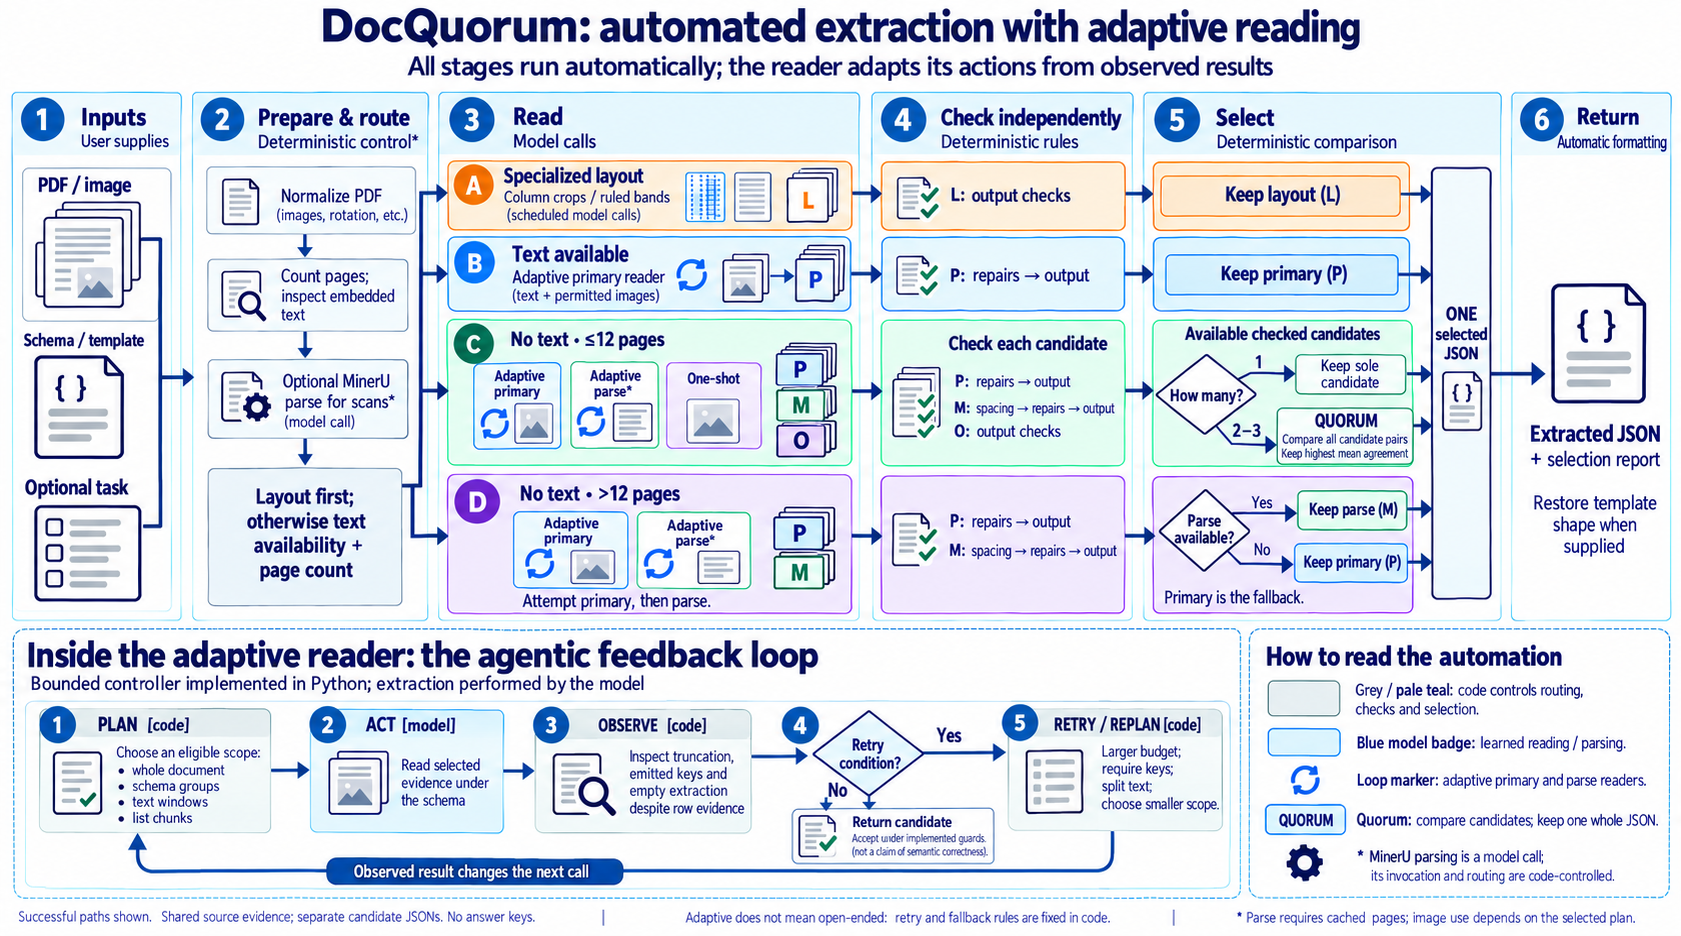
\includegraphics[width=\textwidth,height=6.25cm,keepaspectratio]{assets/pipeline.png}
\src{Pipeline figure (generated with Codex), describing the single-document entry point \texttt{docquorum.extract}; the lower panel shows the reader agent's plan--act--observe loop.}
\end{frame}
\section{Walkthrough on real documents}
\begin{frame}{Step 2: the available evidence decides the route}
\centering
\begin{tabular}{*{5}{>{\centering\arraybackslash}p{0.17\textwidth}}}
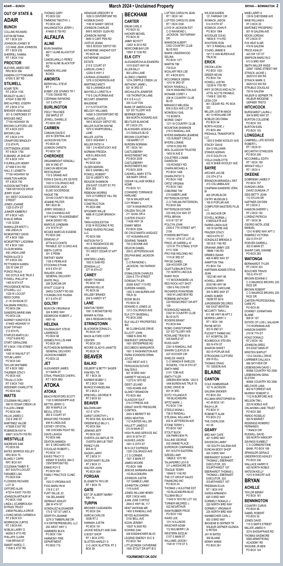
\includegraphics[height=2.1cm,width=0.17\textwidth,keepaspectratio]{assets/route_0.png} & 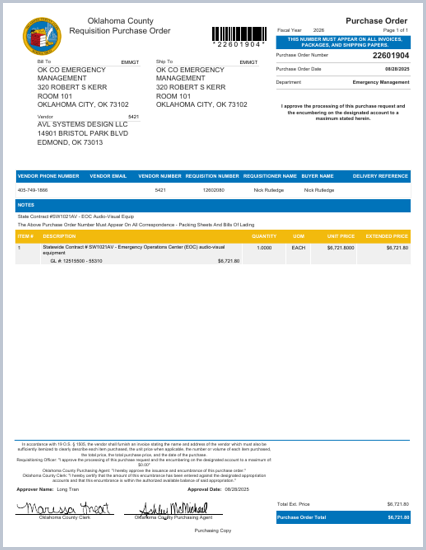
\includegraphics[height=2.1cm,width=0.17\textwidth,keepaspectratio]{assets/route_1.png} & 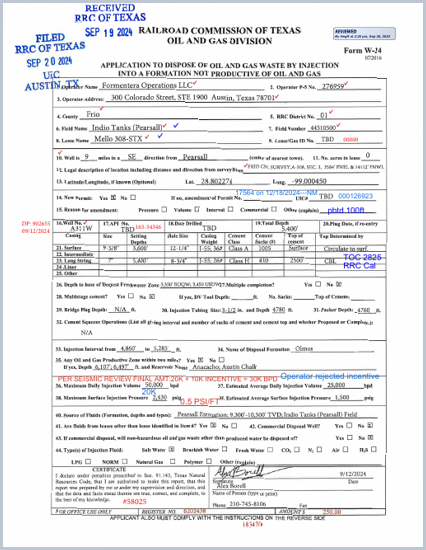
\includegraphics[height=2.1cm,width=0.17\textwidth,keepaspectratio]{assets/route_2.png} & 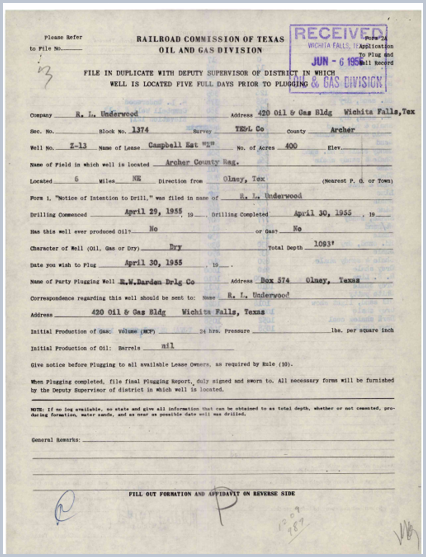
\includegraphics[height=2.1cm,width=0.17\textwidth,keepaspectratio]{assets/route_3.png} & 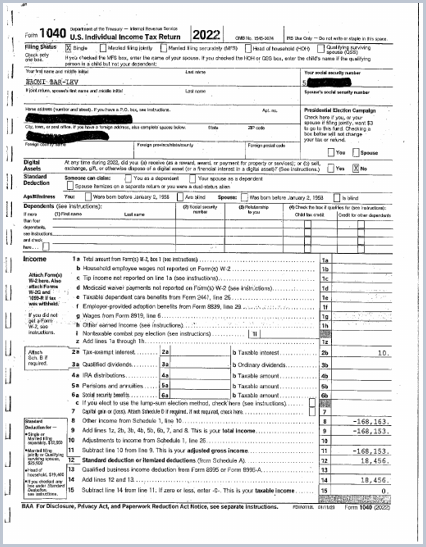
\includegraphics[height=2.1cm,width=0.17\textwidth,keepaspectratio]{assets/route_4.png}\\[0.2em]
{\scriptsize\route{A}\ \textbf{Layout reader}\par}{\tiny Unclaimed-property register\par 59 pages, 15,280 char./page\par} & {\scriptsize\route{B}\ \textbf{Reader agent: text + images}\par}{\tiny County purchase order\par 1 page, 2,253 char./page\par} & {\scriptsize\route{B}\ \textbf{Reader agent: text + images}\par}{\tiny W-14 well form\par 1 page, 252 char./page (OCR layer)\par} & {\scriptsize\route{C}\ \textbf{Three readings, then quorum}\par}{\tiny 1955 plugging application\par 2 pages, no embedded text\par} & {\scriptsize\route{D}\ \textbf{Reader agent on the parse}\par}{\tiny Tax return\par 25 pages, no embedded text\par}
\end{tabular}

\vspace{0.3em}
\begin{block}{Routing rule}
\scriptsize
Layout first: pages printed as equal-width columns of records, or a ruled table on a scan, go to a layout reader \route{A}.
Otherwise a PDF with embedded text (at least 50 characters per page; a digital PDF or an OCR layer) is read once \route{B}.
A scan without text is parsed by MinerU and read three ways if it has at most 12 pages \route{C}, or read through its parse \route{D}.
\end{block}
\src{ExtractBench documents; embedded characters per page measured with pdftotext.}
\end{frame}
\begin{frame}{Step 2: MinerU returns a scanned table as cells}
\begin{columns}[T]
\column{0.41\textwidth}
\textbf{\small Scanned page (detail)}\\[0.3em]
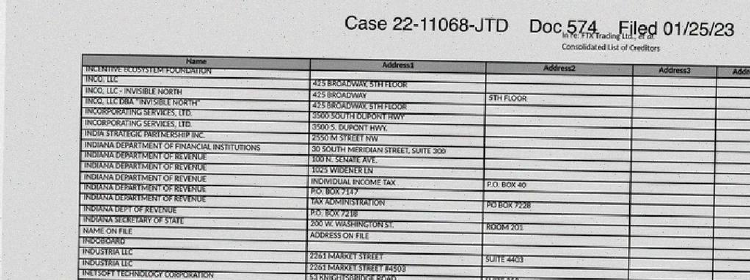
\includegraphics[width=\linewidth]{assets/mineru_page.png}\\[0.5em]
\textbf{\small MinerU output (raw HTML, abbreviated)}\\[0.2em]
\begin{beamercolorbox}[wd=\linewidth,sep=0.4em]{block body}
{\tiny\ttfamily\raggedright <tr><td>Name</td><td>Address1</td><td>Address2...\\<tr><td>INCENTIVE ECOSYSTEM FOUNDATION</td><td...\\<tr><td>INCO, LLC</td><td>425 BROADWAY, 5TH FL...\par}
\end{beamercolorbox}
\column{0.57\textwidth}
\textbf{\small The same rows as table cells (65 rows on this page)}\\[0.3em]
{\tiny \setlength{\tabcolsep}{3pt}\begin{tabular}{@{}>{\raggedright\arraybackslash}p{2.5cm}>{\raggedright\arraybackslash}p{1.9cm}p{1.0cm}p{0.4cm}p{1.0cm}@{}}\toprule
\textbf{Name} & \textbf{Address1} & \textbf{City} & \textbf{State} & \textbf{PostalCode}\\\midrule
INCENTIVE ECOSYSTEM FOUNDATION &  &  &  & \\
INCO, LLC & 425 BROADWAY, 5TH FLOOR &  &  & \\
INO, LLC - INAVAILABLE NORTH & 425 BROADWAY & NEW YORK & NY & 10013\\
INO, LLC DBA "INAVAILABLE NORTH" & 425 BROADWAY, 5TH FLOOR & NEW YORK & NY & 10013-2599\\
INCORPORATING SERVICES, LTD. & 3500 SOUTH COOPONT HWY & NEW YORK & NY & 10013\\
\bottomrule\end{tabular}}

\vspace{0.6em}
{\scriptsize Columns stay aligned: an empty cell stays empty rather than pulling the next value into its place.
Recognition errors remain, so the reader receives the page image together with the parse.\par}
\end{columns}
\src{ExtractBench long: real\_ftx\_full\_corrupted, page 47; cached MinerU2.5 parse.}
\end{frame}
\begin{frame}{Step 3, route \route{A}: the column reader}
\begin{columns}[T]
\column{0.27\textwidth}
\centering
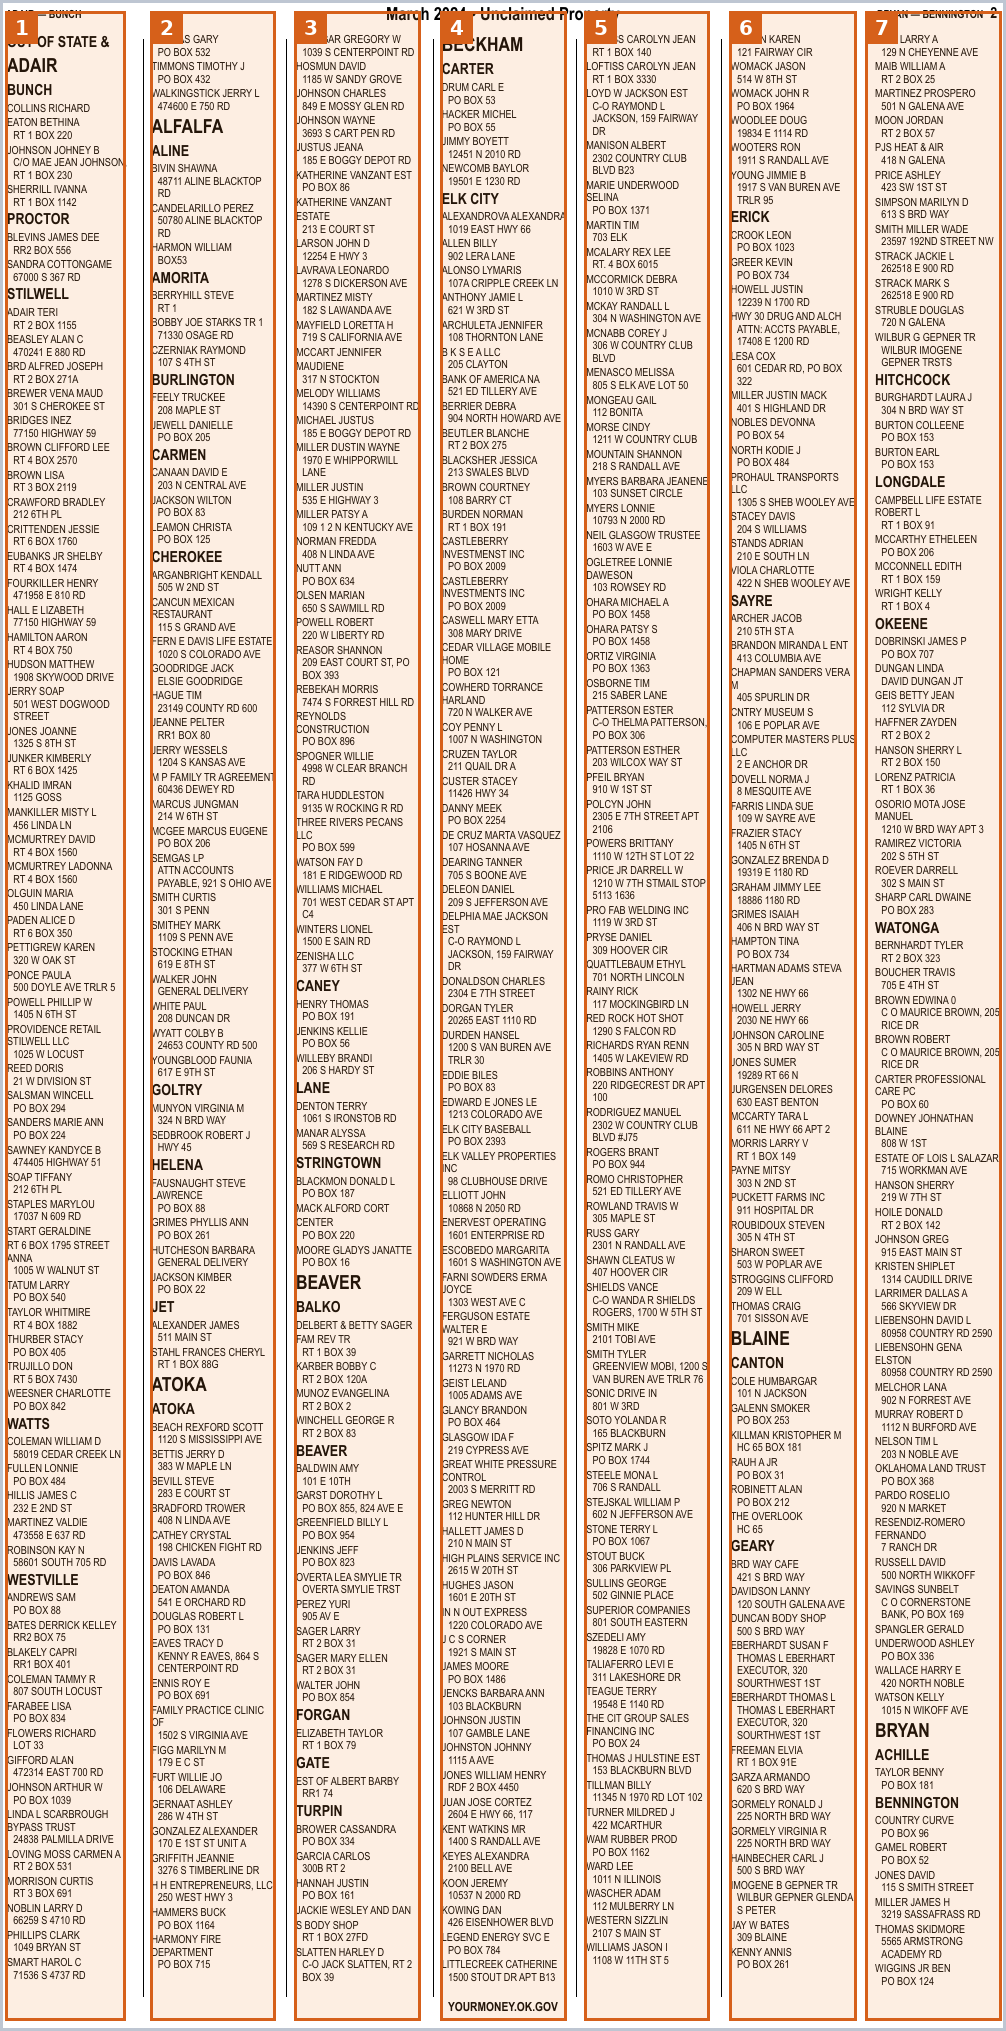
\includegraphics[height=6.1cm]{assets/colflow_page.png}
\column{0.12\textwidth}
\centering
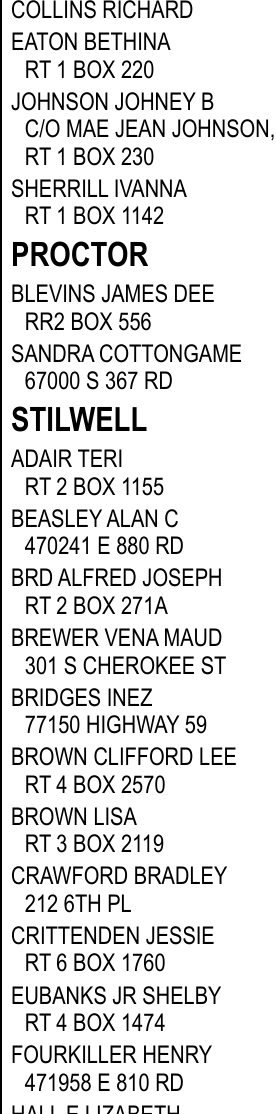
\includegraphics[height=6.1cm]{assets/colflow_crop.png}
\column{0.57\textwidth}
\textbf{\small Records returned for column 1 (page 2)}\\[0.3em]
\begingroup\scriptsize\begin{tabularx}{\linewidth}{@{}p{3.2cm}Y@{}}\toprule
\textbf{name} & \textbf{locale}\\\midrule
\texttt{COLLINS RICHARD} & \texttt{null}\\
\texttt{EATON BETHINA} & \texttt{RT 1 BOX 220}\\
\texttt{JOHNSON JOHNEY B} & \texttt{C/O MAE JEAN JOHNSON, RT 1 BOX 230}\\
\texttt{SHERRILL IVANNA} & \texttt{RT 1 BOX 1142}\\
\bottomrule\end{tabularx}\endgroup

\vspace{0.8em}
\begin{tabular}{@{}lll@{}}
{\Large\bfseries\color{routeA} 7} & {\Large\bfseries\color{routeA} 59} & {\Large\bfseries\color{routeA} 26,675}\\
{\scriptsize columns detected on the page\quad} & {\scriptsize pages\quad} & {\scriptsize records in the final output}
\end{tabular}

\vspace{0.8em}
{\footnotesize The trigger is page geometry only: at least three text columns of near-equal width.
Each column is cut out and read top to bottom in one call; a record continued from the previous column is joined to it.}
\end{columns}
\src{ExtractBench long: real\_oklahoma\_unclaimed\_2024, page 2. Column boxes drawn with the pipeline's own geometry code; records from the stored final output.}
\end{frame}
\begin{frame}{Step 3, route \route{A}: the ruled-table reader}
\begin{columns}[T]
\column{0.52\textwidth}
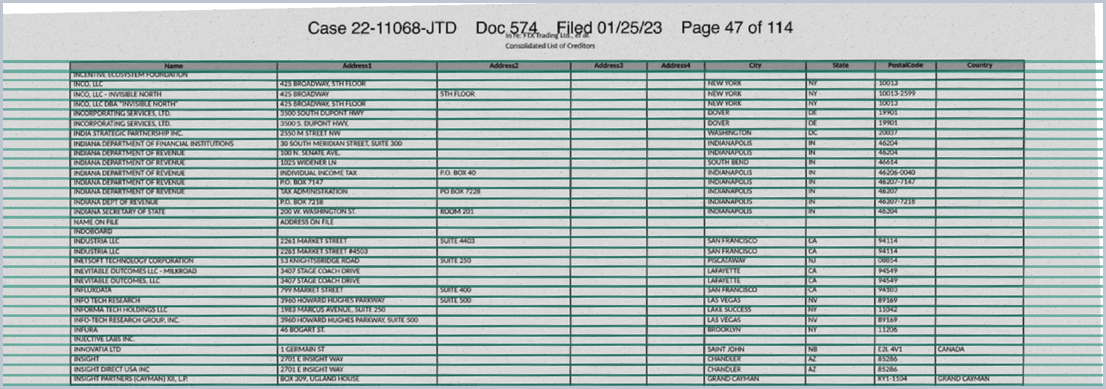
\includegraphics[width=\linewidth]{assets/ruled_page.png}\\[-0.1em]
{\tiny\color{muted} Printed rules detected after deskewing by 1.15$^\circ$ (green).\par}\vspace{0.5em}
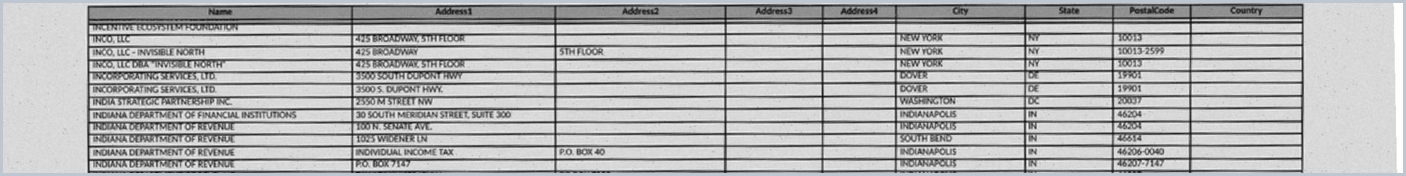
\includegraphics[width=\linewidth]{assets/ruled_band.png}\\[-0.1em]
{\tiny\color{muted} One call: the header row stacked on a band of 12 rows; the reply must contain exactly 12 entries.\par}
\column{0.45\textwidth}
\begin{tabular}{@{}ll@{}}
{\Large\bfseries\color{routeA} 67} & {\Large\bfseries\color{routeA} 67}\\
{\scriptsize rows counted from the rules\quad} & {\scriptsize rows returned by the reader}
\end{tabular}

\vspace{0.4em}
{\footnotesize Bands on page 47: 12 + 12 + 12 + 12 + 12 + 7.}

\vspace{0.5em}
\begingroup\tiny\begin{tabularx}{\linewidth}{@{}Yp{1.9cm}p{1.0cm}p{0.5cm}@{}}\toprule
\textbf{name} & \textbf{address\_1} & \textbf{city} & \textbf{state}\\\midrule
\texttt{INCENTIVE ECOSYSTEM FOUNDATION} & \texttt{null} & \texttt{null} & \texttt{null}\\
\texttt{INCO, LLC} & \texttt{425 BROADWAY, 5TH FLOOR} & \texttt{NEW YORK} & \texttt{NY}\\
\texttt{INCO, LLC - INVISIBLE NORTH} & \texttt{425 BROADWAY} & \texttt{NEW YORK} & \texttt{NY}\\
\bottomrule\end{tabularx}\endgroup

\vspace{0.5em}
{\footnotesize Fixing the number of entries per band prevents repeated identical rows from multiplying or disappearing.}
\end{columns}
\src{ExtractBench long: real\_ftx\_full\_corrupted, page 47. Rows from the stored final output.}
\end{frame}
\begin{frame}{Step 3, route \route{C}: three independent readings of one scan}
\begin{columns}[T]
\column{0.24\textwidth}
\centering
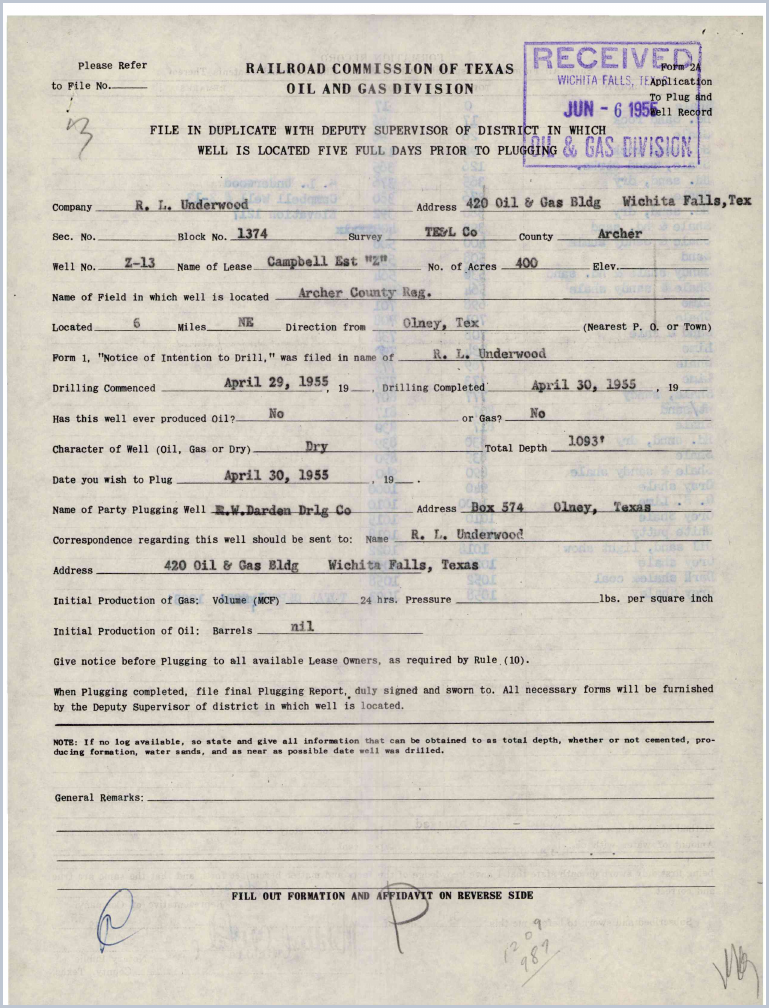
\includegraphics[width=\linewidth]{assets/input_form_p1.png}
\column{0.74\textwidth}
\begingroup\scriptsize\begin{tabularx}{\linewidth}{@{}p{3.1cm}YYp{1.6cm}@{}}\toprule
\textbf{field} & \cand{P}{routeB}\ \textbf{image reading} & \cand{M}{routeC}\ \textbf{parse reading} & \cand{O}{routeD}\ \textbf{one-shot}\\\midrule
\texttt{p1\_company} & \texttt{R. L. Underwood} & \texttt{R. L. Underwood} & \nul\\
\texttt{p1\_county} & \texttt{Archer} & \texttt{Archer} & \nul\\
\texttt{p1\_well\_no} & \texttt{Z-13} & \texttt{Z-13} & \nul\\
\texttt{p1\_name\_of\_lease} & \texttt{Campbell Est "Z"} & \texttt{Campbell Est "Z"} & \nul\\
\texttt{p1\_drilling\_commenced} & \texttt{April 29, 1955} & \texttt{April 29, 1955} & \nul\\
\texttt{p1\_party\_plugging\_well} & \textcolor{bad}{\texttt{R.W. Darden Dr'lg Co}} & \textcolor{bad}{\texttt{R.W.Darden Drlg Co}} & \nul\\
\texttt{p2\_correspondence\_name} & \textcolor{bad}{\texttt{R.L. Underwood}} & \textcolor{bad}{\texttt{R.L.Underwood}} & \nul\\
\bottomrule\end{tabularx}\endgroup

\vspace{0.3em}
{\tiny\color{muted} Red: empty, or the two readings disagree (P and M differ only in spacing and punctuation).}

\vspace{0.6em}
\begin{tabular}{@{}lll@{}}
\cand{P}{routeB}\ {\large\bfseries 59\,/\,77}\qquad & \cand{M}{routeC}\ {\large\bfseries 59\,/\,77}\qquad & \cand{O}{routeD}\ {\large\bfseries 1\,/\,77}\\
{\scriptsize fields filled} & {\scriptsize fields filled} & {\scriptsize fields filled}
\end{tabular}

\vspace{0.5em}
{\footnotesize P: the reader agent on the page images. M: the reader agent on the MinerU parse and the images. O: the benchmark's own one-shot reader.}
\end{columns}
\src{ExtractBench short: 2A-9-160298\_109929; stored readings after their checks.}
\end{frame}
\begin{frame}{Step 4: checks that repair the structure of a reading}
\begingroup\scriptsize\renewcommand{\arraystretch}{1.12}
\begin{tabularx}{\textwidth}{@{}>{\raggedright\arraybackslash}p{2.9cm}>{\raggedright\arraybackslash}p{3.0cm}Y>{\raggedleft\arraybackslash}p{1.9cm}@{}}\toprule
\textbf{Check} & \textbf{Document} & \textbf{Observed change} & \textbf{Value F1}\\\midrule
\textbf{Rows copied into another list} & Pueblo check register (medium) & \textcolor{good}{\textbf{562\,$\rightarrow$\,51 batch rows}}\newline{\tiny Check 01033982 (\$700.88) had also been filed as a batch with the same number and amount.} & 84.73\,$\rightarrow$\,99.91\\[0.1em]
\textbf{Identical records capped at the printed count} & FTX creditor list, text layer (long) & \textcolor{good}{\textbf{146\,$\rightarrow$\,37 rows on page 59}}\newline{\tiny Page 59 prints the line ``NAME ON FILE'' exactly 37 times.} & 84.47\,$\rightarrow$\,90.77\\[0.1em]
\textbf{Stacked lines folded into one record} & Clinical adverse-event listing (long) & \textcolor{good}{\textbf{1,499\,$\rightarrow$\,668 records}}\newline{\tiny Subject R1002: three printed lines became one event with its resolved date.} & 38.80\,$\rightarrow$\,68.77\\[0.1em]
\textbf{Template rows dropped} & Texas W-14 well form (short) & \textcolor{good}{\textbf{5\,$\rightarrow$\,2 casing rows}}\newline{\tiny Three rows carried only the printed row label (e.g.\ ``Intermediate'').} & 82.30\,$\rightarrow$\,93.23\\[0.1em]
\bottomrule\end{tabularx}\endgroup

\vspace{0.3em}
{\tiny Examples are the cases each check was designed for. On a few short documents some repairs lowered the score slightly (e.g.\ duplicate removal on three election reports, $-$3.5 points in total).\par}
\src{Stored readings before and after each check, re-run with \texttt{docquorum/checks} and scored with ExtractBench's scorer. Each check uses only the schema and the document's own text; no model is called.}
\end{frame}
\begin{frame}{Step 4: checks that make values exactly what the page prints}
\begingroup\scriptsize\renewcommand{\arraystretch}{1.12}
\begin{tabularx}{\textwidth}{@{}>{\raggedright\arraybackslash}p{2.9cm}>{\raggedright\arraybackslash}p{3.0cm}Y>{\raggedleft\arraybackslash}p{1.9cm}@{}}\toprule
\textbf{Check} & \textbf{Document} & \textbf{Observed change} & \textbf{Value F1}\\\midrule
\textbf{Every schema field present} & Caterpillar 330 spec sheet (short) & \textcolor{good}{\textbf{missing keys\,$\rightarrow$\,\texttt{null}}}\newline{\tiny The reply omitted 7 optional fields in every specification row; the scorer counts an absent key as a miss.} & 61.48\,$\rightarrow$\,95.74\\[0.1em]
\textbf{A blank tick box is false} & Texas P-4 form (short) & \textcolor{good}{\textbf{6 boxes: \texttt{null}\,$\rightarrow$\,\texttt{false}}}\newline{\tiny The field description states ``false if left blank''.} & 91.67\,$\rightarrow$\,96.67\\[0.1em]
\textbf{Quotes as printed} & Census statistical table (short) & \textcolor{good}{\textbf{Bachelor\textquotesingle{}s\,$\rightarrow$\,Bachelor's}}\newline{\tiny The page prints a typographic apostrophe; only the quote character is copied from the page.} & 60.12\,$\rightarrow$\,62.58\\[0.1em]
\textbf{Numbers as printed} & Schedule K-1 (short, one-shot reading) & \textcolor{good}{\textbf{33.333333\,$\rightarrow$\,33.3333333}}\newline{\tiny A rounded value is replaced by the single printed figure it restates (6 share fields).} & 85.42\,$\rightarrow$\,97.92\\[0.1em]
\bottomrule\end{tabularx}\endgroup

\vspace{0.3em}
{\tiny Every replacement is a value that the document itself prints, or \texttt{null} where the schema admits null.\par}
\src{Stored readings before and after each check, re-run with \texttt{docquorum/checks} and scored with ExtractBench's scorer. Each check uses only the schema and the document's own text; no model is called.}
\end{frame}
\begin{frame}{Step 5: selection by quorum}
\begin{columns}[T]
\column{0.42\textwidth}
\centering
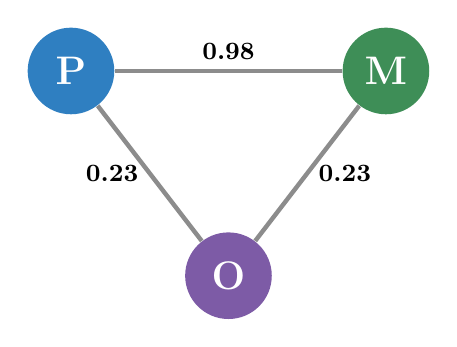
\begin{tikzpicture}[every node/.style={font=\small}]
\node[circle,fill=routeB,text=white,minimum size=1.1cm,font=\Large\bfseries] (P) at (0,2.6) {P};
\node[circle,fill=routeC,text=white,minimum size=1.1cm,font=\Large\bfseries] (M) at (4,2.6) {M};
\node[circle,fill=routeD,text=white,minimum size=1.1cm,font=\Large\bfseries] (O) at (2,0) {O};
\draw[line width=1.6pt,black!45] (P) -- node[above,black]{\textbf{0.98}} (M);
\draw[line width=1.6pt,black!45] (P) -- node[left,black]{\textbf{0.23}} (O);
\draw[line width=1.6pt,black!45] (M) -- node[right,black]{\textbf{0.23}} (O);
\end{tikzpicture}

\vspace{0.6em}
{\scriptsize Edge: agreement of two readings, measured with the benchmark's value scorer, recall-weighted ($F_{\beta}$, $\beta=2$).\par}
\column{0.55\textwidth}
{\footnotesize\begin{tabular}{@{}lrl@{}}\toprule
\textbf{Reading} & \textbf{Mean agreement} & \\\midrule
\rowcolor{hl}\cand{P}{routeB}\ image reading & 0.604 & \textbf{kept}\\
\cand{M}{routeC}\ parse reading & 0.604 & \\
\cand{O}{routeD}\ one-shot & 0.218 & \\\bottomrule
\end{tabular}}

\vspace{0.4em}
{\scriptsize P and M tie; ties go to the reading listed first. The whole of P is returned; fields are never mixed across readings.}

\vspace{0.6em}
\begin{block}{Agreement is not accuracy}
\scriptsize
Answer-key value F1 for this document (illustration only; never used by the pipeline): P 95.24, M 95.24, O 22.50.
On the scanned county purchase order the quorum kept the one-shot reading (78.26), although the image reading scored higher (82.61).
\end{block}
\end{columns}
\src{ExtractBench short: 2A-9-160298\_109929; agreement computed by \texttt{docquorum.quorum.pick} on the checked readings.}
\end{frame}
\begin{frame}{Step 6: one checked JSON, in the form requested}
\begin{columns}[T]
\column{0.47\textwidth}
\textbf{\small JSON Schema in, JSON out (1955 form, 77 fields)}\\[0.3em]
\begin{beamercolorbox}[wd=\linewidth,sep=0.5em]{block body}
{\scriptsize\ttfamily\raggedright \{\\\hspace*{1.04em}\textquotedbl{}p1\_company\textquotedbl{}: \textquotedbl{}R. L. Underwood\textquotedbl{},\\\hspace*{1.04em}\textquotedbl{}p1\_address\textquotedbl{}: \textquotedbl{}420 Oil \& Gas Bldg Wichita Falls, Tex\textquotedbl{},\\\hspace*{1.04em}\textquotedbl{}p1\_county\textquotedbl{}: \textquotedbl{}Archer\textquotedbl{},\\\hspace*{1.04em}\textquotedbl{}p1\_well\_no\textquotedbl{}: \textquotedbl{}Z-13\textquotedbl{},\\\hspace*{1.04em}\textquotedbl{}p1\_name\_of\_lease\textquotedbl{}: \textquotedbl{}Campbell Est \textbackslash{}\textquotedbl{}Z\textbackslash{}\textquotedbl{}\textquotedbl{},\\\hspace*{1.04em}\textquotedbl{}p1\_drilling\_commenced\textquotedbl{}: \textquotedbl{}April 29, 1955\textquotedbl{},\\\hspace*{1.04em}\textquotedbl{}p1\_total\_depth\textquotedbl{}: \textquotedbl{}1093\textquotesingle{}\textquotedbl{},\\\hspace*{1.04em}... 70 further fields\\\}\par}
\end{beamercolorbox}
\column{0.50\textwidth}
\textbf{\small JSON template in, the same template filled}\\[0.3em]
\begin{columns}[T]
\column{0.32\linewidth}
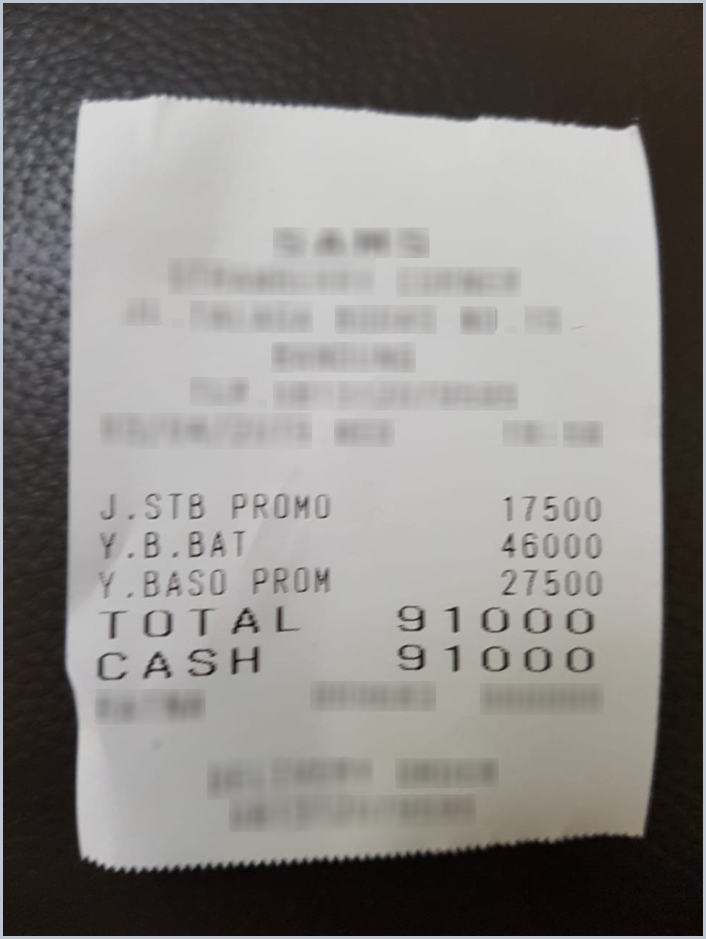
\includegraphics[width=\linewidth]{assets/input_receipt.png}
\column{0.66\linewidth}
{\tiny\color{muted} Template}\\
{\tiny\ttfamily\raggedright \{\textquotedbl{}menu\textquotedbl{}: [\{\textquotedbl{}price\textquotedbl{}: \textquotedbl{}\textquotedbl{}, \textquotedbl{}nm\textquotedbl{}: \textquotedbl{}\textquotedbl{}\}],\\\hspace*{0.52em}\textquotedbl{}total\textquotedbl{}: \{\textquotedbl{}cashprice\textquotedbl{}: \textquotedbl{}\textquotedbl{},\\\hspace*{5.72em}\textquotedbl{}total\_price\textquotedbl{}: \textquotedbl{}\textquotedbl{}\}\}\par}\vspace{0.6em}
{\tiny\color{muted} Output (equal to the answer key)}\\
{\tiny\ttfamily\raggedright \{\textquotedbl{}menu\textquotedbl{}: [\\\hspace*{1.56em}\{\textquotedbl{}price\textquotedbl{}: \textquotedbl{}17500\textquotedbl{}, \textquotedbl{}nm\textquotedbl{}: \textquotedbl{}J.STB PROMO\textquotedbl{}\},\\\hspace*{1.56em}\{\textquotedbl{}price\textquotedbl{}: \textquotedbl{}46000\textquotedbl{}, \textquotedbl{}nm\textquotedbl{}: \textquotedbl{}Y.B.BAT\textquotedbl{}\},\\\hspace*{1.56em}\{\textquotedbl{}price\textquotedbl{}: \textquotedbl{}27500\textquotedbl{}, \textquotedbl{}nm\textquotedbl{}: \textquotedbl{}Y.BASO PROM\textquotedbl{}\},\\\hspace*{0.52em}],\\\hspace*{0.52em}\textquotedbl{}total\textquotedbl{}: \{\textquotedbl{}cashprice\textquotedbl{}: \textquotedbl{}91000\textquotedbl{},\\\hspace*{5.72em}\textquotedbl{}total\_price\textquotedbl{}: \textquotedbl{}91000\textquotedbl{}\}\}\par}
\end{columns}
\end{columns}
\src{Left: stored final output for 2A-9-160298\_109929. Right: UNIKIE-BENCH Catering-Services test\_1.jpg, quorum over six stored readings.}
\end{frame}
\section{Results}
\begin{frame}{ExtractBench: complete results (1/3)}
\begingroup\scriptsize\renewcommand{\arraystretch}{1.0}\setlength{\tabcolsep}{5pt}
\begin{tabularx}{\textwidth}{@{}rYlrrrr@{}}\toprule
\textbf{\#} & \textbf{System} & \textbf{Type} & \textbf{Short} & \textbf{Medium} & \textbf{Long} & \textbf{Overall}\\\midrule
1 & LlamaExtract Agentic Plus & Commercial service & 96.94 & 94.45 & 90.18 & 95.91\\
1 & Pulse (Effort) & Commercial service & 96.46 & 95.01 & 93.51 & 95.91\\
\rowcolor{hl}\textbf{3} & \textbf{DocQuorum (ours)} & \textbf{Open model (27B)} & \textbf{96.34} & \textbf{94.11} & \textbf{90.41} & \textbf{95.43}\\
4 & LlamaExtract Agentic & Commercial service & 96.04 & 92.11 & 91.83 & 94.77\\
5 & Codex (GPT-6 Sol Evidence) & Coding agent & 95.99 & 92.42 & 87.25 & 94.57\\
6 & Codex (GPT-5.6 Sol Evidence) & Coding agent & 96.04 & 90.19 & 82.73 & 93.77\\
7 & Codex (GPT-5.5) & Coding agent & 95.68 & 91.15 & 78.88 & 93.57\\
8 & Codex (GPT-5.5 Evidence) & Coding agent & 95.59 & 88.72 & 87.97 & 93.35\\
9 & Pulse (Non-effort) & Commercial service & 93.17 & 92.22 & 89.07 & 92.70\\
10 & LlamaExtract Cost-Effective & Commercial service & 94.03 & 89.51 & 83.73 & 92.27\\
11 & Codex (GPT-5.6 Terra Evidence) & Coding agent & 95.60 & 86.69 & 77.36 & 92.26\\
12 & OpenAI GPT-6 Astra & Commercial model & 97.22 & 90.56 & 31.70 & 91.91\\
13 & Codex (GPT-5.6 Luna Evidence) & Coding agent & 93.50 & 87.43 & 80.05 & 91.16\\
14 & Codex (GPT-6 Luna Evidence) & Coding agent & 93.09 & 87.71 & 80.88 & 91.01\\
15 & Reducto Deep Extract & Commercial service & 94.20 & 80.47 & 92.01 & 90.44\\
16 & Qwen3.8 Flash Next & Open model & 94.82 & 87.81 & 37.74 & 89.88\\
\bottomrule\end{tabularx}\endgroup
\src{ExtractBench leaderboard, snapshot of 2 October 2026 (47 published systems) and DocQuorum. Value F1 (\%) by the benchmark's scorer over 370 PDFs (252 short, 98 medium, 20 long); Overall is the mean over all documents. Equal scores share a rank.}
\end{frame}
\begin{frame}{ExtractBench: complete results (2/3)}
\begingroup\scriptsize\renewcommand{\arraystretch}{1.0}\setlength{\tabcolsep}{5pt}
\begin{tabularx}{\textwidth}{@{}rYlrrrr@{}}\toprule
\textbf{\#} & \textbf{System} & \textbf{Type} & \textbf{Short} & \textbf{Medium} & \textbf{Long} & \textbf{Overall}\\\midrule
17 & Qwen3.8 27B & Open model & 94.68 & 87.54 & 38.45 & 89.75\\
18 & Extend (Max Context) & Commercial service & 92.32 & 78.75 & 90.46 & 88.62\\
19 & Qwen3.6 35B & Open model & 92.86 & 86.37 & 36.90 & 88.11\\
20 & Qwen3.5 35B & Open model & 93.52 & 85.27 & 31.73 & 88.00\\
21 & DeepSeek V4.1 Flash & Commercial model & 94.44 & 81.49 & 22.23 & 87.11\\
22 & Claude Code (Opus 4.8) & Coding agent & 90.08 & 79.21 & 88.07 & 87.09\\
23 & Claude Code (Opus 4.8 Evidence) & Coding agent & 90.54 & 79.17 & 77.94 & 86.84\\
24 & Qwen3.5 9B & Open model & 92.31 & 81.12 & 32.22 & 86.10\\
25 & Claude Code (Opus 5.5 Evidence) & Coding agent & 89.63 & 77.96 & 80.83 & 86.06\\
26 & Extend Extract & Commercial service & 89.39 & 84.14 & 47.21 & 85.72\\
27 & Datalab (Accurate + Balanced) & Commercial service & 89.40 & 85.08 & 42.04 & 85.70\\
28 & Reducto Extract & Commercial service & 92.97 & 69.59 & 30.65 & 83.41\\
29 & Kimi K3 & Commercial model & 94.64 & 69.64 & 4.99 & 83.17\\
30 & Qwen3.5 4B & Open model & 89.06 & 76.64 & 27.31 & 82.43\\
31 & NuExtract3 & Open model & 86.41 & 77.01 & 32.71 & 81.02\\
32 & GLM-5.3 Flash & Commercial model & 96.30 & 51.56 & 27.83 & 80.75\\
\bottomrule\end{tabularx}\endgroup
\src{ExtractBench leaderboard, snapshot of 2 October 2026 (47 published systems) and DocQuorum. Value F1 (\%) by the benchmark's scorer over 370 PDFs (252 short, 98 medium, 20 long); Overall is the mean over all documents. Equal scores share a rank.}
\end{frame}
\begin{frame}{ExtractBench: complete results (3/3)}
\begingroup\scriptsize\renewcommand{\arraystretch}{1.0}\setlength{\tabcolsep}{5pt}
\begin{tabularx}{\textwidth}{@{}rYlrrrr@{}}\toprule
\textbf{\#} & \textbf{System} & \textbf{Type} & \textbf{Short} & \textbf{Medium} & \textbf{Long} & \textbf{Overall}\\\midrule
33 & Google Gemini 3.8 Flash & Commercial model & 88.14 & 72.23 & 28.70 & 80.71\\
34 & Google Gemini 3.5 Flash & Commercial model & 87.87 & 69.76 & 27.90 & 79.84\\
35 & Lift Datalab 9B & Open model & 87.64 & 65.69 & 24.78 & 78.43\\
36 & OpenAI GPT-5.4 Nano & Commercial model & 77.43 & 76.37 & 35.81 & 74.90\\
37 & Gemma4 26B & Open model & 77.70 & 59.61 & 28.88 & 70.27\\
38 & Gemma4 E4B & Open model & 81.10 & 48.93 & 26.82 & 69.64\\
39 & InternVL3.5 14B & Open model & 80.70 & 39.04 & 19.41 & 66.35\\
40 & InternVL3.5 8B & Open model & 79.26 & 36.62 & 17.57 & 64.63\\
41 & Qwen3.5 2B & Open model & 71.22 & 50.93 & 25.93 & 63.40\\
42 & Kimi-VL A3B & Open model & 69.86 & 34.61 & 18.94 & 57.77\\
43 & Gemma4 E2B & Open model & 63.71 & 28.96 & 14.58 & 51.85\\
44 & NuExtract 2.0 8B & Open model & 62.92 & 23.50 & 6.39 & 49.42\\
45 & Qwen3.5 0.8B & Open model & 57.44 & 26.98 & 6.65 & 46.63\\
46 & MiniCPM-V 4.5 & Open model & 57.39 & 25.30 & 1.13 & 45.85\\
47 & Gemma4 12B & Open model & 53.62 & 30.82 & 13.16 & 45.39\\
48 & GLM-4.6V Flash & Open model & 47.28 & 44.52 & 22.17 & 45.19\\
\bottomrule\end{tabularx}\endgroup
\src{ExtractBench leaderboard, snapshot of 2 October 2026 (47 published systems) and DocQuorum. Value F1 (\%) by the benchmark's scorer over 370 PDFs (252 short, 98 medium, 20 long); Overall is the mean over all documents. Equal scores share a rank.}
\end{frame}
\begin{frame}{UNIKIE-BENCH: complete results}
\begingroup\scriptsize\renewcommand{\arraystretch}{0.9}\setlength{\tabcolsep}{3.2pt}
\begin{tabularx}{\textwidth}{@{}rYc*{11}{r}r@{}}\toprule
\textbf{\#} & \textbf{System} & & \textbf{Ret.} & \textbf{Cat.} & \textbf{Com.} & \textbf{Acc.} & \textbf{Post.} & \textbf{Adm.} & \textbf{Edu.} & \textbf{Adv.} & \textbf{Tax} & \textbf{Med.} & \textbf{Nut.} & \textbf{Avg.}\\\midrule
\rowcolor{hl}1 & \textbf{DocQuorum (ours)} & O & \textbf{\underline{90.63}} & \textbf{\underline{88.13}} & \textbf{53.51} & \textbf{79.29} & \textbf{85.65} & \textbf{\underline{87.00}} & \textbf{85.67} & \textbf{86.59} & \textbf{\underline{82.16}} & \textbf{\underline{78.33}} & \textbf{92.22} & \textbf{\underline{82.65}}\\
2 & Gemini-3-Pro & C & 89.27 & 83.54 & \underline{53.87} & \underline{81.43} & \underline{90.74} & 84.32 & 80.71 & \underline{90.54} & 81.54 & 77.60 & \underline{92.47} & 82.37\\
3 & Qwen3-VL-Plus & C & 89.12 & 86.45 & 50.57 & 77.86 & 83.55 & 78.91 & \underline{87.44} & 83.14 & 78.93 & 76.46 & 89.72 & 80.20\\
4 & Qwen3-VL-8B & O & 88.26 & 86.23 & 51.14 & 71.07 & 83.80 & 78.90 & 87.39 & 81.23 & 78.74 & 77.19 & 86.36 & 79.12\\
5 & Qwen-VL-Max & C & 86.67 & 84.68 & 49.33 & 76.07 & 84.85 & 79.96 & 82.46 & 82.76 & 77.94 & 75.62 & 75.14 & 77.77\\
6 & GLM-4.1V-9B & O & 62.32 & 77.33 & 46.67 & 76.43 & 76.46 & 78.75 & 65.83 & 81.99 & 70.68 & 72.08 & 60.47 & 69.91\\
7 & GPT-4o & C & 75.79 & 79.33 & 49.67 & 67.86 & 82.95 & 64.26 & 47.77 & 73.56 & 75.33 & 67.57 & 76.51 & 69.15\\
8 & MiMo-VL-7B-RL & O & 77.45 & 77.66 & 49.01 & 67.50 & 76.70 & 76.81 & 76.65 & 66.28 & 74.86 & 68.70 & 46.10 & 68.88\\
9 & InternVL3.5-8B & O & 77.23 & 72.23 & 41.64 & 67.14 & 73.90 & 72.10 & 63.08 & 73.08 & 72.81 & 65.94 & 65.53 & 67.70\\
10 & GPT-5 & C & 71.90 & 71.33 & 45.94 & 69.29 & 80.95 & 62.79 & 50.26 & 75.48 & 72.05 & 67.71 & 75.83 & 67.59\\
11 & MiniCPM-V4.5-8B & O & 68.37 & 74.91 & 45.91 & 67.76 & 83.60 & 71.89 & 63.21 & 79.31 & 69.57 & 70.00 & 44.18 & 67.15\\
12 & Claude-Sonnet-4.5 & C & 69.24 & 73.65 & 45.92 & 69.29 & 79.45 & 69.20 & 39.46 & 85.06 & 67.79 & 63.96 & 67.24 & 66.39\\
13 & Kimi-VL-A3B & O & 86.49 & 63.12 & 42.87 & 61.79 & 83.40 & 68.72 & 80.37 & 72.41 & 77.80 & 64.93 & 25.72 & 66.14\\
14 & Gemma-3-12B & O & 54.32 & 68.73 & 30.68 & 53.93 & 72.30 & 37.14 & 17.56 & 36.78 & 56.81 & 48.54 & 52.20 & 48.09\\
15 & Ministral-3-8B & O & 6.47 & 57.01 & 26.24 & 43.39 & 75.80 & 32.37 & 29.54 & 19.53 & 65.85 & 51.46 & 6.17 & 37.62\\
16 & SmolVLM2-2.2B & O & 17.80 & 57.22 & 28.52 & 18.92 & 34.98 & 8.63 & 3.87 & 27.16 & 34.97 & 18.00 & 10.51 & 23.69\\
\bottomrule\end{tabularx}\endgroup

\vspace{0.3em}
{\tiny Ret.\ Retail; Cat.\ Catering services; Com.\ Commercial; Acc.\ Accommodation; Post.\ Postal label; Adm.\ Administrative; Edu.\ Education; Adv.\ Advertisement; Tax: Tax-compliant; Med.\ Medical services; Nut.\ Nutrition label; Avg.\ macro average. C: closed model; O: open model. Underlined: best in the column.\par}
\src{UNIKIE-BENCH (ACL 2026), Table 4: 15 published systems; F1 (\%) by the benchmark's evaluator on 4,472 images, every input capped at 1,605,632 pixels. DocQuorum: quorum over six readings from three open models; small images enlarged before reading.}
\end{frame}
\begin{frame}{Results on six benchmarks}
\begingroup\footnotesize\renewcommand{\arraystretch}{1.25}
\begin{tabularx}{\textwidth}{@{}Yrll@{}}\toprule
\textbf{Benchmark} & \textbf{DocQuorum} & \textbf{Place} & \textbf{Comparison}\\\midrule
\rowcolor{hl}VAREX (1,777 government forms) {\footnotesize(with zoom re-reading)} & \textbf{98.23} & \textbf{1st of 21} & next: Gemini 2.5 Pro 98.0\\
\rowcolor{hl}UNIKIE-BENCH (4,472 images) {\footnotesize(with zoom re-reading)} & \textbf{82.65} & \textbf{1st of 16} & next: Gemini-3-Pro 82.37\\
LongArray-Extract (45 long documents) & \textbf{98.05} & 2nd of 12 & 1st: Extend MAX 99.2\\
UNIKIE-BENCH open category (1,661 documents) {\footnotesize(with zoom re-reading)} & \textbf{72.33} & 2nd of 16 & 1st: Gemini-3-Pro 81.65\\
ExtractBench (370 PDFs) {\footnotesize(development set)} & \textbf{95.43} & 3rd of 48 & 1st: LlamaExtract Agentic Plus 95.91\\
DocuBench (72 documents, 10 file types) & \textbf{90.80} & 4th of 10 & 1st: DocuPipe (high effort) 97.02\\
\bottomrule\end{tabularx}\endgroup

\vspace{0.6em}
{\small Each score is the benchmark's own scorer on the full test set, with open-weight models (Qwen3.8-27B and MinerU2.5) on one GPU. Places count every published system.\par}
\src{docs/results/: one complete table per benchmark (TABLES.md). No result was submitted to a leaderboard.}
\end{frame}
\begin{frame}{Zoom re-reading: a new step after the quorum}
\begin{columns}[T]
\column{0.52\textwidth}
\small
After the quorum keeps one reading, each field on which the readings disagree is found on the page and read once more from a sharp crop of that region.\par\vspace{0.5em}
This new reading sees none of the earlier answers. It changes the kept value only if it matches a value some reading already proposed, and it counts as two votes: it can overturn a lead of one reading, not a clear majority.\par\vspace{0.5em}
The vote rule was added after the third test, where five agreeing readings were overturned too often.
\column{0.44\textwidth}
\begin{block}{Three tests}
\small
VAREX: 98.10\,$\rightarrow$\,\textbf{98.30}\\
60 forms better, 25 worse\\[0.5em]
UNIKIE open: 71.07\,$\rightarrow$\,\textbf{72.33}\\
291 documents better, 138 worse\\[0.5em]
UNIKIE (six readings): 82.62\,$\rightarrow$\,81.62; 82.65 with the vote rule
\end{block}
\end{columns}
\src{results/README.md: method, statistics, and every changed value checked against the answer key after the runs.}
\end{frame}
\section{Summary}
\begin{frame}{Summary}
\begin{columns}[T]
\column{0.32\textwidth}
\begin{block}{Results}
\small
1st on VAREX and UNIKIE-BENCH; 2nd on LongArray-Extract and UNIKIE open; 3rd on ExtractBench.\\[0.4em]
A new step, zoom re-reading, improved VAREX and UNIKIE open; with its vote rule it holds UNIKIE level.\\[0.4em]
Open-weight models on one GPU.
\end{block}
\column{0.32\textwidth}
\begin{block}{Method}
\small
Routing by the available evidence; an agentic reader that plans, reads and re-reads; layout readers for column flow and ruled tables; deterministic checks against the schema and the page; selection by quorum.
\end{block}
\column{0.32\textwidth}
\begin{block}{Limitations}
\small
ExtractBench served as the development set. Agreement among readings does not guarantee accuracy. Checks are triggered by schema wording and page text; a few repairs lower the score on some documents.
\end{block}
\end{columns}
\end{frame}
\end{document}
